\documentclass[12pt,a4paper]{article}

\usepackage[utf8]{inputenc}
\usepackage[T1]{fontenc}
\usepackage[english]{babel}
\usepackage{geometry}
\usepackage{longtable}
\usepackage{tabularx}
\usepackage{array}
\usepackage{booktabs}
\usepackage{listings}
\usepackage{xcolor}
\usepackage{hyperref}
\usepackage{enumitem}
\usepackage{float}
\usepackage{graphicx}
\usepackage{ragged2e}
\usepackage{graphicx}
\usepackage{float}


\newcolumntype{P}[1]{>{\RaggedRight\arraybackslash}p{#1}}

\geometry{margin=2.2cm}
\setlength{\parskip}{0.5em}
\setlength{\parindent}{0pt}
\setlength{\LTleft}{0pt}
\setlength{\LTright}{0pt}

\hypersetup{
    colorlinks=true,
    linkcolor=black,
    urlcolor=blue
}

\lstset{
    basicstyle=\ttfamily\small,
    breaklines=true,
    frame=single,
    columns=fullflexible
}

\title{\textbf{Homework 3 --- Multi-Process Word Transportation and Concurrent Sorting System}\\
GTU CSE344 System Programming}
\author{Dicle Çoban}
\date{April 15, 2026}

\begin{document}

\maketitle
\thispagestyle{empty}

\section*{Cover Information}

\begin{tabularx}{\textwidth}{>{\bfseries}l X}
Course & CSE344 --- System Programming \\
Homework & Homework 3 --- Multi-Process Word Transportation and Concurrent Sorting System \\
Submission Date & 2026-04-15 \\
Student & Dicle Çoban \\
Language & C (POSIX-compatible, multi-process implementation) \\
\end{tabularx}

\vspace{1em}

\section{Introduction}

This homework implements a multi-process word transportation and concurrent sorting system in C on a POSIX-compatible environment. The system reads words from an input text file, admits them to arrival floors, transports their characters one by one to sorting floors, and reconstructs the original words concurrently.

The goal of the homework is not only to move data from one place to another, but to manage concurrent access to shared data structures correctly. Multiple independent processes may attempt to claim words, claim character tasks, update sorting areas, and use elevator subsystems at the same time. Therefore, the main design challenges are:

\begin{itemize}[leftmargin=1.5em]
\item safe shared-memory usage,
\item synchronization of all concurrent updates,
\item prevention of duplicate work,
\item atomic floor-capacity admission,
\item coordinated completion detection,
\item and clean process termination.
\end{itemize}

\section{System Architecture}

\subsection{Overall Architecture}

The implementation is centered around one parent/coordinator process and multiple child processes that cooperate through a shared memory region created with \texttt{mmap(..., MAP\_SHARED | MAP\_ANONYMOUS, ...)}. The system consists of six active subsystems:

\begin{itemize}[leftmargin=1.5em]
\item \textbf{Parent / Coordinator Process}: parses arguments, reads input, initializes shared state and synchronization objects, spawns all child processes, monitors completion, writes the final output file, prints summary information, and performs shutdown.
\item \textbf{Word-Carrier Processes}: fixed to their initial floor; scan the input list in synchronized round-robin order and admit words only when capacity rules are satisfied.
\item \textbf{Letter-Carrier Processes}: mobile worker processes; claim one character at a time and either directly place it or request elevator transportation.
\item \textbf{Sorting Processes}: fixed to a sorting floor; incrementally reconstruct words using sorting metadata, fixed positions, moves, and swaps.
\item \textbf{Delivery Elevator Process}: handles character transportation requests.
\item \textbf{Reposition Elevator Process}: handles relocation requests of idle letter-carrier processes.
\end{itemize}

\subsection{Process Responsibilities}

\begin{longtable}{|P{3.8cm}|P{11.2cm}|}
\hline
\textbf{Process Type} & \textbf{Responsibility} \\
\hline
Parent / Coordinator & Initializes the system, creates all child processes, monitors completion, generates output, prints final statistics, handles shutdown and cleanup. \\
\hline
Word-Carrier & Scans the input list in round-robin order, atomically claims a candidate word, checks arrival-floor and sorting-floor capacity, admits or releases the word. \\
\hline
Letter-Carrier & Claims one character task from the current floor, uses direct placement or delivery elevator, remains at destination floor after delivery, requests reposition when idle. \\
\hline
Sorting Process & Works on words assigned to its own floor, fixes correct positions, moves misplaced characters, performs swaps, and marks words as completed. \\
\hline
Delivery Elevator & Serves character delivery requests through the delivery queue and wakes the corresponding letter-carrier after delivery completes. \\
\hline
Reposition Elevator & Serves idle-carrier movement requests through the reposition queue and wakes the corresponding letter-carrier after relocation. \\
\hline
\end{longtable}

\section{Data Structures and Shared Memory Design}

\subsection{Shared State Overview}

All process-visible state is placed inside a single shared \texttt{SharedState} structure. This structure contains:

\begin{itemize}[leftmargin=1.5em]
\item global configuration and counters,
\item all words loaded from the input file,
\item per-floor information,
\item per-carrier state,
\item per-sorter and per-word-carrier statistics,
\item delivery and reposition request queues,
\item and all synchronization primitives used between processes.
\end{itemize}

\subsection{SharedWord Structure}

Each word is represented by a \texttt{SharedWord} structure. It stores:

\begin{itemize}[leftmargin=1.5em]
\item \texttt{word\_id},
\item original \texttt{text},
\item \texttt{sorting\_floor},
\item \texttt{arrival\_floor},
\item \texttt{claimed}, \texttt{admitted}, and \texttt{completed} flags,
\item \texttt{sorting\_area[]},
\item \texttt{sorting\_meta[]},
\item \texttt{occupied[]},
\item \texttt{fixed[]},
\item per-character state arrays such as \texttt{char\_claimed[]}, \texttt{char\_delivered[]}, \texttt{char\_in\_transit[]}, and \texttt{char\_arrived[]}.
\end{itemize}

The \texttt{sorting\_meta[]} array stores the original index of the character currently occupying a sorting slot. This is the key structure that allows correct reconstruction, including repeated characters.

\subsection{Other Shared Structures}

\begin{longtable}{|P{3.6cm}|P{11.4cm}|}
\hline
\textbf{Structure} & \textbf{Purpose} \\
\hline
\texttt{FloorState} & Stores the current number of active words and the current letter-carrier count on each floor. \\
\hline
\texttt{CarrierState} & Stores a carrier's current floor, statistics, and private event semaphore information used to block and wake that carrier. \\
\hline
\texttt{DeliveryRequest} & Represents a pending character delivery request: source floor, destination floor, word index, character index, and carrier slot. \\
\hline
\texttt{RepositionRequest} & Represents a pending reposition request for an idle carrier. \\
\hline
\end{longtable}

\section{Synchronization Strategy}

The implementation uses POSIX named semaphores and shared-memory synchronization. The main synchronization objects are:

\begin{itemize}[leftmargin=1.5em]
\item \texttt{global\_mutex}: protects globally shared metadata such as the round-robin cursor and slot allocation.
\item Per-floor mutexes: protect \texttt{active\_words} and \texttt{carrier\_count}.
\item Per-word mutexes: protect claim flags, delivery state, sorting area updates, completion flags, and word-local consistency.
\item \texttt{sorter\_lock} per word: ensures only one sorting process works on a specific word at a time.
\item \texttt{delivery\_mutex} and \texttt{reposition\_mutex}: protect the two elevator request queues.
\item \texttt{delivery\_items} and \texttt{reposition\_items}: counting semaphores used to wake elevator processes when queued work exists.
\item \texttt{parent\_event}: wakes the parent when important global events occur.
\item \texttt{word\_available\_sem}: used by word-carrier processes when they must wait for future admission opportunities.
\item Private carrier event semaphores: used by elevator processes to wake the correct letter-carrier after delivery or reposition.
\end{itemize}

\subsection{Race Condition Prevention}

Race conditions are prevented by combining shared memory with explicit critical sections:

\begin{itemize}[leftmargin=1.5em]
\item word claiming is synchronized under the global mutex,
\item admission checks lock the relevant floor mutexes in increasing floor order,
\item character-task claiming is protected by the word mutex,
\item sorting-area updates are also protected by the word mutex,
\item same-word concurrent sorting is blocked by the per-word sorter lock.
\end{itemize}

\subsection{Critical Sections}

The most important critical sections are:

\begin{itemize}[leftmargin=1.5em]
\item round-robin cursor update and word claim,
\item floor-capacity admission and reservation,
\item character-task claim / delivery state update,
\item sorting-area move or swap operations,
\item word completion and floor-capacity release,
\item queue insertion for delivery and reposition requests.
\end{itemize}

\section{Word Admission Logic}

Word-carrier processes implement synchronized round-robin scanning. A shared round-robin cursor points to the next candidate position in the input list. When a word-carrier starts a scan:

\begin{enumerate}[leftmargin=1.5em]
\item it acquires the global mutex,
\item it searches from the current cursor position for an unclaimed, not-yet-admitted, not-yet-completed word,
\item it marks that word as claimed atomically,
\item it advances the shared cursor,
\item it releases the global mutex.
\end{enumerate}

Then the process checks admission. Admission is accepted only if:

\begin{itemize}[leftmargin=1.5em]
\item the arrival floor has capacity,
\item the sorting floor has capacity.
\end{itemize}

This check is performed atomically by locking the two floor mutexes in a deterministic order. If both checks succeed, the capacities are reserved immediately and the word becomes admitted. If either check fails, the word is released and may be selected again later. This implements the all-or-nothing admission policy required by the homework.

\section{Character Transportation and Elevators}

\subsection{Character Tasks}

Each word is decomposed implicitly by using the original text and per-character arrays. A letter-carrier process scans admitted words on its current floor and selects exactly one character such that:

\begin{itemize}[leftmargin=1.5em]
\item it is not already claimed,
\item it is not already delivered,
\item it is not already in transit.
\end{itemize}

When such a character is found, the carrier marks it as claimed and in transit under the word mutex.

\subsection{Delivery Rules}

If the sorting floor is equal to the carrier's current floor, the carrier directly places the character into the word's sorting area. Otherwise, it creates a delivery request and waits on its private event semaphore until the delivery elevator completes the request.

After a successful delivery:

\begin{itemize}[leftmargin=1.5em]
\item the character is placed into the sorting area,
\item its delivery flag is updated,
\item the carrier's current floor becomes the destination floor,
\item the carrier continues execution from that floor.
\end{itemize}

\subsection{Delivery Elevator}

The delivery elevator maintains its own independent request queue. It wakes when delivery requests exist, collects a batch up to its configured capacity, processes the requests, updates delivery statistics, and signals the corresponding carriers after each request is completed.

\subsection{Reposition Elevator}

If a letter-carrier finds no available task on its current floor, it requests reposition to a random floor. The reposition elevator handles these requests through a separate queue and separate synchronization primitives. After relocation, the carrier resumes execution from its new floor.

\subsection{Idle-Carrier Recovery}

The parent process also monitors floors with zero active letter-carriers. If a floor becomes empty and the system is not yet complete, the parent respawns the configured number of letter-carriers for that floor. This prevents total disappearance of workers from a floor.

\section{Sorting Algorithm}

Characters are not inserted directly to their final positions. Instead, each delivered character is first placed into the first suitable non-fixed empty slot in \texttt{sorting\_area[]}. The corresponding \texttt{sorting\_meta[]} entry records the original index of that character in the word.

The sorting process works as follows:

\begin{itemize}[leftmargin=1.5em]
\item If the slot is empty, it does nothing.
\item If the slot is fixed, it does nothing.
\item If the character's original index matches the current slot index, it marks that slot as fixed.
\item If the target slot is empty, it moves the character there.
\item If the target slot is occupied and not fixed, it swaps the two entries.
\item If the target slot is fixed, it leaves the character unchanged for a future pass.
\end{itemize}

This design satisfies the required move/swap rules. Because each character keeps its original index through \texttt{sorting\_meta[]}, repeated letters are handled correctly and do not become ambiguous.

\section{Termination Detection}

Word completion is detected by checking whether all entries of \texttt{fixed[]} are equal to 1. When a word completes:

\begin{itemize}[leftmargin=1.5em]
\item its \texttt{completed} flag is set,
\item the global completed-word counter is incremented,
\item the reserved capacity on arrival and sorting floors is released,
\item a wake-up is sent to the parent if all words are complete.
\end{itemize}

The parent waits on \texttt{parent\_event} while monitoring \texttt{completed\_words}. Once all words are complete, the parent:

\begin{enumerate}[leftmargin=1.5em]
\item sets the global shutdown flag,
\item wakes blocked processes,
\item creates the final output file,
\item prints summary statistics,
\item waits for all child processes,
\item releases resources.
\end{enumerate}

The program also installs \texttt{SIGINT} and \texttt{SIGTERM} handlers so that Ctrl+C triggers a controlled shutdown path.

\section{Output File Generation}

\textbf{Output verification:}
After each execution, the produced output file was compared with the corresponding input file. 
The verification process checked four conditions: 
(1) every input word appeared exactly once in the output, 
(2) the original \texttt{sorting\_floor} value of each word was preserved, 
(3) the output file contained no blank or malformed lines, and 
(4) the final ordering matched the assignment specification, namely sorting first by \texttt{sorting\_floor} and then by \texttt{word\_id}. 
This verification confirmed that the final output was both complete and correctly ordered.


The output file is generated only after all words have been completed. The parent first creates an array of pointers to shared words and sorts it by:




\begin{enumerate}[leftmargin=1.5em]
\item \texttt{sorting\_floor},
\item \texttt{word\_id}.
\end{enumerate}

Then each line is written in the exact required format:

\begin{lstlisting}
<word_id> <word> <sorting_floor>
\end{lstlisting}

No blank line is written. The arrival floor does not affect the final output. Therefore, the final file preserves the original word and sorting-floor information while enforcing the required ordering rule.

\section{Test Case Scenario}

\subsection{Mandatory Test Case}

The produced output file is shown directly below the summary. 
It preserves all input words, keeps the original sorting-floor values, and is ordered by sorting floor and word id as required.
The following test case was used to validate the basic functionality of the system.

\textbf{Run command:}
\begin{lstlisting}
./hw3 -f 3 -w 2 -l 2 -s 2 -c 5 -d 8 -r 5 -i sample_input.txt -o output.txt
\end{lstlisting}

\textbf{Input file screenshot:}
\begin{figure}[H]
    \centering
    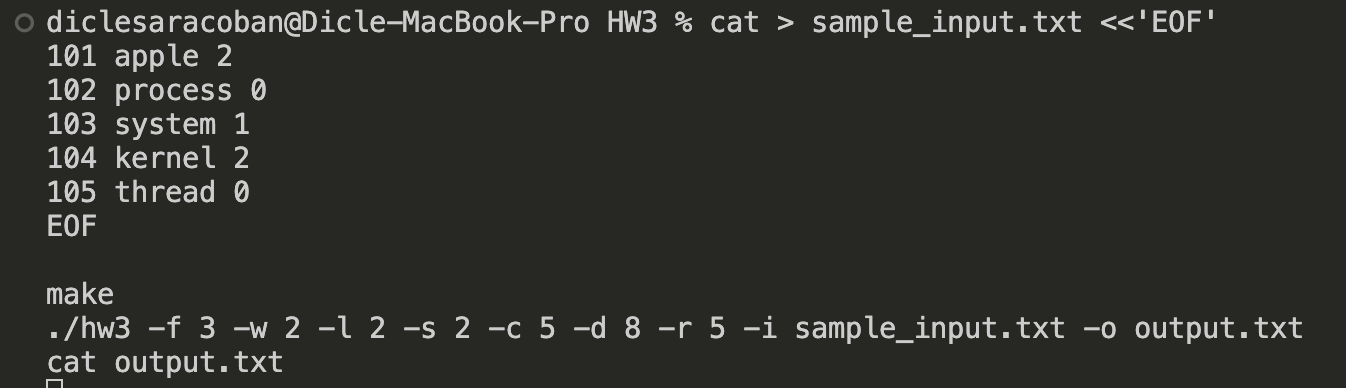
\includegraphics[width=0.92\textwidth]{input1.png}
    \caption{Mandatory test case input file}
\end{figure}

\textbf{Output / summary screenshot:}
\begin{figure}[H]
    \centering
    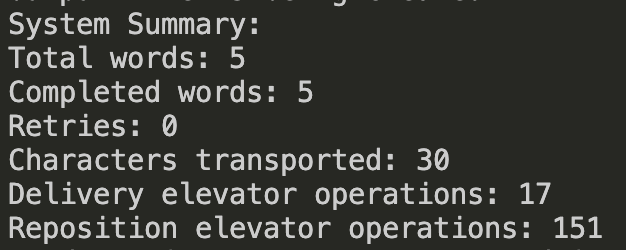
\includegraphics[width=0.7\textwidth]{output1.png}
    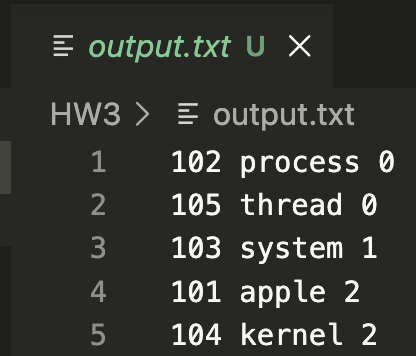
\includegraphics[width=0.7\textwidth]{outputTxt.png}
    \caption{Mandatory test case summary and output}
\end{figure}

\textbf{Observed behavior:}
\begin{itemize}[leftmargin=1.5em]
\item The program initialized multiple process types on each floor.
\item Words were admitted only when both arrival-floor and sorting-floor capacities were available.
\item Characters were transported concurrently and reconstructed on their sorting floors.
\item The final output file was produced in the required order.
\end{itemize}

\subsection{Large Input Test}

This test was used to observe the behavior of the system under a larger workload.

\textbf{Run command:}
\begin{lstlisting}
./hw3 -f 6 -w 2 -l 3 -s 2 -c 10 -d 10 -r 5 -i input_big.txt -o output_big.txt
\end{lstlisting}

\textbf{Input file screenshot:}
\begin{figure}[H]
    \centering
    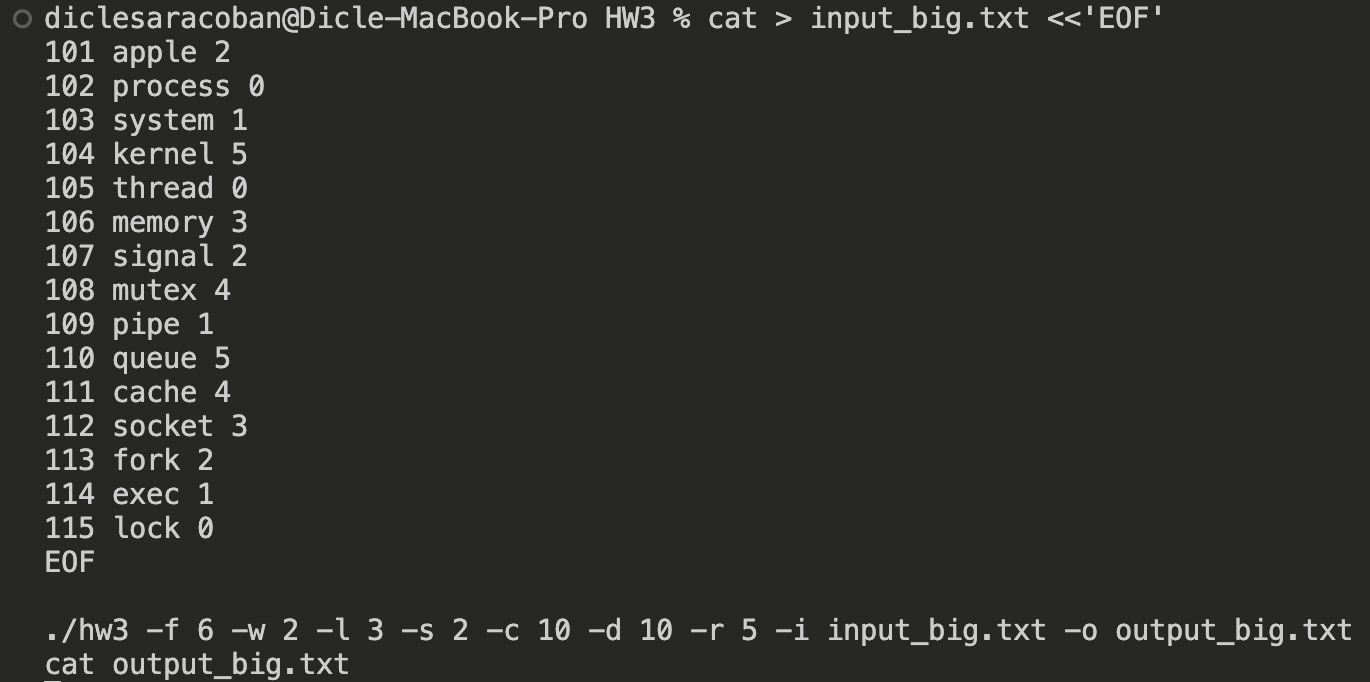
\includegraphics[width=0.92\textwidth]{input2.png}
    \caption{Large input test file}
\end{figure}

\textbf{Output / summary screenshot:}
\begin{figure}[H]
    \centering
    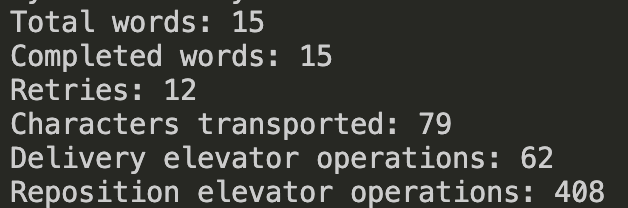
\includegraphics[width=0.7\textwidth]{output2.png}
    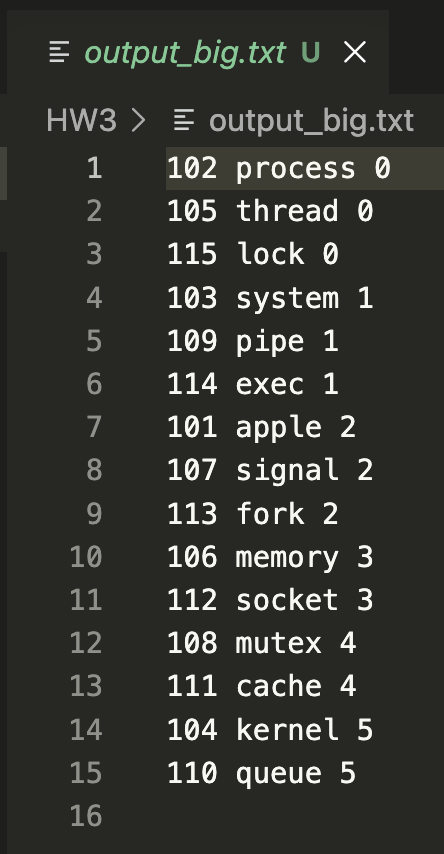
\includegraphics[width=0.7\textwidth]{outputBigTxt.png}
    \caption{Large input test summary and output}
\end{figure}

\textbf{Observed behavior:}
\begin{itemize}[leftmargin=1.5em]
\item The system completed all words successfully under a larger input size.
\item The sorting order of the final output remained correct.
\item Retry count increased compared to the basic case because more words competed for resources.
\end{itemize}

\subsection{Mini Input Test}

This smaller test case was used for quick verification of correctness.

\textbf{Run command:}
\begin{lstlisting}
./hw3 -f 2 -w 1 -l 1 -s 1 -c 3 -d 3 -r 2 -i mini_input.txt -o mini_output.txt
\end{lstlisting}

\textbf{Input file screenshot:}
\begin{figure}[H]
    \centering
    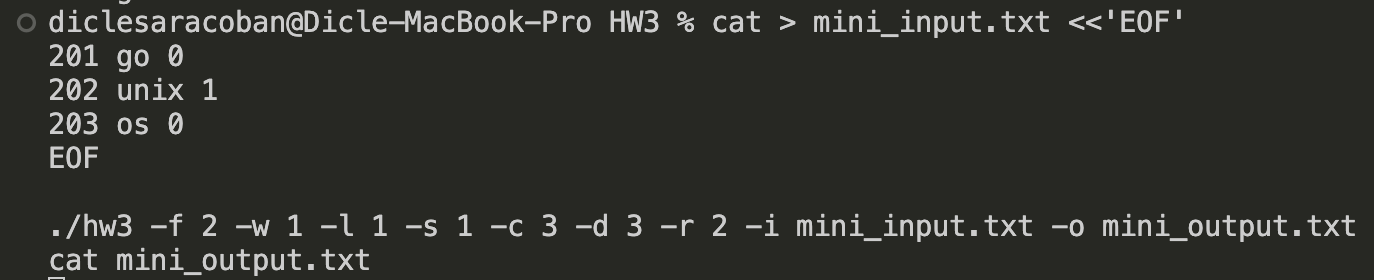
\includegraphics[width=0.92\textwidth]{input3.png}
    \caption{Mini input test file}
\end{figure}

\textbf{Output / summary screenshot:}
\begin{figure}[H]
    \centering
    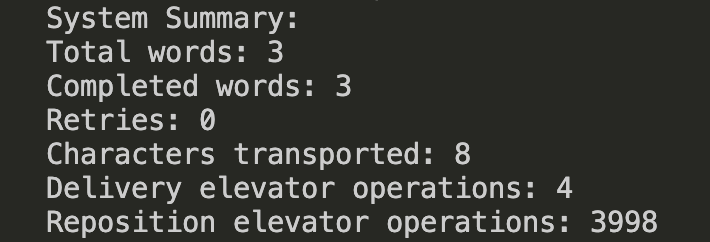
\includegraphics[width=0.7\textwidth]{output3.png}
    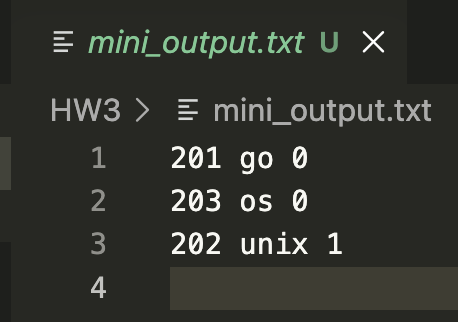
\includegraphics[width=0.7\textwidth]{miniOutputTxt.png}
    \caption{Mini input test summary and output}
\end{figure}

\textbf{Observed behavior:}
\begin{itemize}[leftmargin=1.5em]
\item The system handled a very small workload correctly.
\item The final output order matched the expected sorting-floor and word-id ordering.
\item This test was useful for quick debugging and sanity checking.
\end{itemize}

\section{Challenges and Solutions}

The implementation was challenging mainly because several process groups modify related shared state concurrently. The most important problems and solutions were:

\begin{longtable}{|P{4.0cm}|P{10.8cm}|}
\hline
\textbf{Challenge} & \textbf{Solution} \\
\hline
Duplicate word claims & Protected round-robin scan and claim operations with the global mutex. \\
\hline
Inconsistent admission state & Performed atomic dual-floor capacity checking with deterministic lock order. \\
\hline
Concurrent sorting on the same word & Added a per-word sorter lock in addition to the per-word mutex. \\
\hline
Duplicate character delivery risk & Used per-character claim, in-transit, delivered, and arrived flags under the word mutex. \\
\hline
Idle-carrier coordination & Added reposition requests and a dedicated reposition elevator queue. \\
\hline
Termination detection & Used completed flags and a completed-word counter monitored by the parent. \\
\hline
Cross-process wake-up of respawned carriers & Introduced carrier-specific named event semaphores that can be reopened safely after process creation. \\
\hline
\end{longtable}




\section{Conclusion}

This homework required the integration of process creation, shared memory, synchronization, queue-based subsystem coordination, and system-wide termination logic. The final design uses a shared-memory state model, per-word and per-floor synchronization, and separate delivery/reposition elevator queues to keep the system correct under concurrency.

The implementation satisfies the core assignment requirements: words are admitted atomically, characters are delivered exactly once, sorting is protected from concurrent corruption, the output file is generated after system completion, and the parent process performs coordinated shutdown and cleanup.

\end{document}
